\section{Môi trường}

    Môi khi một biến nào đó được tạo ra, chúng cần phải được lưu trữ trong một môi trường. \textbf{Môi trường} là một cấu trúc dữ liệu lưu trữ thông tin về các biến và các hàm, cũng như về phạm vi truy cập của chúng. Trong trình thông dịch Pandora, môi trường được sử dụng trong giai đoạn phân tích ngữ nghĩa và thông dịch. Dưới đây là vị trí mà  môi trường được sử dụng trong trình thông dịch Pandora:

\begin{figure}[H]
    \centering
    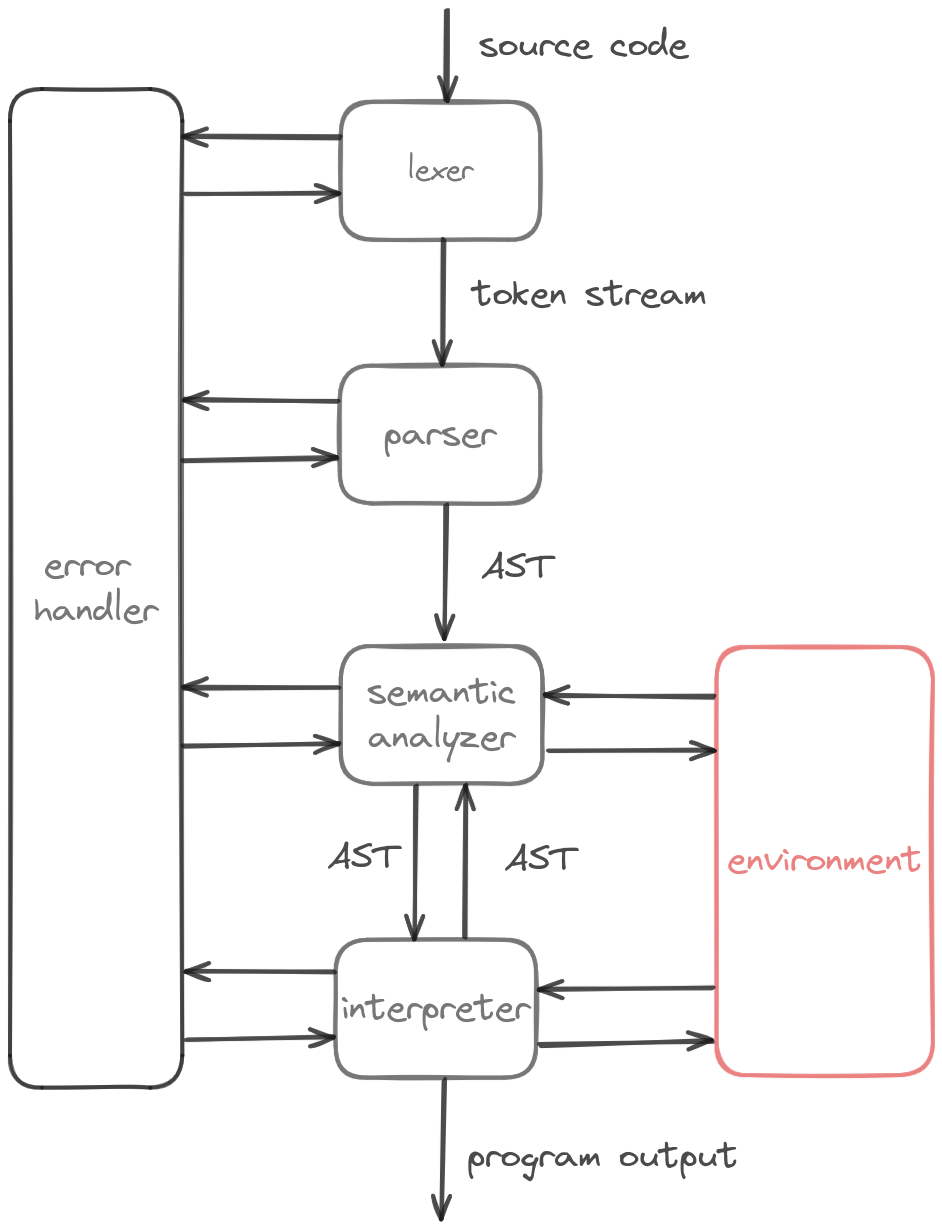
\includegraphics[scale=0.4]{env-pos.png}
    \caption{Môi trường trong cấu trúc của trình thông dịch Pandora}
\end{figure}

\noindent Cấu trúc môi trường trong Pandora được định nghĩa như sau:

\begin{lstlisting}[]
pub struct Environment {
    pub scopes: Vec<Scope>,
    pub in_function: bool,
    pub default_libs: HashMap<String, Box<dyn Library>>,
}
\end{lstlisting}

    Trong đó:
    \begin{itemize}
        \item \texttt{scopes} là một vector chứa các phạm vi, mỗi phạm vi là một \texttt{Scope}.
        \item \texttt{in\_function} là một biến boolean xác định xem trình thông dịch đang ở trong một hàm hay không.
        \item \texttt{default\_libs} là một bảng băm chứa các thư viện mặc định của Pandora.
    \end{itemize}

    \textbf{Phạm vi} là một cấu trúc dữ liệu lưu trữ thông tin về các biến và hàm, cũng như về phạm vi truy cập của chúng. Trong Pandora, phạm vi biến được sử dụng để lưu trữ thông tin về các biến và hàm trong một phạm vi cụ thể. Dưới đây là cấu trúc của phạm vi biến trong Pandora:

\begin{lstlisting}[]
pub struct Scope {
    pub variables: Vec<Wrapper<Variable>>,
    pub libraries: HashMap<String, (Span, Box<dyn Library>)>,
    pub functions: HashMap<String, (Span, ValueKind)>,      
}
\end{lstlisting}

    Trong đó:
    \begin{itemize}
        \item \texttt{variables} là một vector chứa tthông tin về các biến được khai báo trong phạm vi biến, bao gồm vị trí khai báo và biến.
        \item \texttt{libraries} là một bảng băm chứa thông tin về các thư viện được thêm vào phạm vi biến, bao gồm vị trí thêm và thư viện.
        \item \texttt{functions} là một bảng băm chứa thông tin về các hàm được định nghĩa trong phạm vi biến, bao gồm vị trí khai báo và loại hàm.
    \end{itemize}

    Phạm vi sẽ lưu trữ một số thông tin cơ bản của biến như tên biến, kiểu dữ liệu, giá trị, vị trí gán đầu tiên, và một số thông tin khác. Dưới đây là cấu trúc của biến trong Pandora:

\begin{lstlisting}[]
pub struct Variable {
    pub ident: Ident,
    pub is_mut: bool,
    pub val: Option<Value>,
    pub ty: Ty,
    pub first_assigned_span: Option<Span>,
}
\end{lstlisting}

    Ta để ý thấy rằng, phạm vi sẽ lưu thông tin các biến dưới dạng vector, trong đó mỗi phần tử của vector là một biến, trong khi đó lại lưu thông tin về thư viện và hàm dưới dạng bảng băm. Sở dĩ như vậy là vì trong ngôn ngữ Pandora, người dùng được phép khai báo nhiều biến trùng tên trong cùng một phạm vi (kỹ thuật này được gọi là \textbf{shadowing}), nhưng không được phép thêm nhiều thư viện hoặc khai báo nhiều hàm trùng tên trong cùng một phạm vi. Do đó, việc lưu trữ thông tin về biến dưới dạng vector sẽ giúp ta dễ dàng thêm, sửa, xóa thông tin về biến, trong khi việc lưu trữ thông tin về thư viện và hàm dưới dạng bảng băm sẽ giúp ta dễ dàng kiểm tra xem một thư viện hoặc hàm đã được thêm vào phạm vi một cách nhanh chóng.

    Đối với hàm, ta sẽ lưu thông tin về hàm dưới dạng bảng băm, trong đó key của bảng băm là tên hàm, value của bảng băm là một tuple gồm vị trí khai báo và hàm thực thi (evaluation function), sẵn sàng để được gọi khi cần.  

    Đối với thư viện, ta cũng lưu thông tin về thư viện dưới dạng bảng băm, trong đó key của bảng băm là tên thư viện, value của bảng băm là một tuple gồm vị trí thêm và thư viện:

\begin{lstlisting}[]
pub trait Library {
    fn get_function(
        &self,
        name: &str,
    ) -> Option<&Box<dyn Fn(CallerAttrs, Vec<(Value, bool)>) -> Result<ValueKind, Vec<IError>>>>;
}
\end{lstlisting}

    Mỗi thư viện sẽ cung cấp một phương thức \texttt{get\_function} để lấy thông tin về hàm trong thư viện. Phương thức này sẽ trả về một hàm thực thi (evaluation function) dựa trên tên hàm được truyền vào.

    Như đã nói ở trên, do người dùng chỉ được phép thêm một thư viện hoặc khai báo một hàm trùng tên trong cùng một phạm vi, nên việc lưu trữ thông tin về thư viện và hàm dưới dạng bảng băm sẽ giúp ta dễ dàng kiểm tra xem một thư viện hoặc hàm đã được thêm vào phạm vi một cách nhanh chóng.

    Với cấu trúc phạm vi như trên, trình thông dịch Pandora sẽ dễ dàng kiểm tra xem một biến, thư viện hay hàm đã được khai báo hay thêm vào phạm vi chưa, cũng như lấy thông tin về chúng một cách nhanh chóng.

    Như vậy, môi trường sẽ lưu một danh sách các phạm vi, mỗi phạm vi sẽ lưu thông tin về các biến, thư viện và hàm được khai báo hoặc thêm vào phạm vi đó. Danh sách phạm vi được xếp theo thứ tự từ phạm vi lớn nhất đến phạm vi nhỏ nhất, với phạm vi cuối cùng là phạm vi nhỏ nhất cũng là phạm vi hiện tại. Khi trình thông dịch cần truy cập thông tin về một biến, thư viện hoặc hàm, nó sẽ bắt đầu tìm kiếm từ phạm vi hiện tại, nếu không tìm thấy, nó sẽ tiếp tục tìm kiếm ở các phạm vi lớn hơn cho đến khi tìm thấy hoặc hết phạm vi. Mỗi khi truy cập vào một khối lệnh, trình thông dịch sẽ tạo một phạm vi mới và thêm vào danh sách phạm vi, khi ra khỏi khối lệnh, trình thông dịch sẽ xóa phạm vi cuối cùng khỏi danh sách phạm vi. Điều này giúp trình thông dịch Pandora duy trì thông tin về các biến, thư viện và hàm trong quá trình thực thi chương trình. Riêng đối với trường hợp truy cập vào một hàm để thực thi các lệnh trong hàm đó, trình thông dịch sẽ tạo một môi trường mới cho hàm đó. Thuộc tính \texttt{in\_function} trong môi trường sẽ giúp trình thông dịch nhận biết xem nó đang ở trong một hàm hay không, hỗ trợ cho việc soát ngữ nghĩa và thực thi chương trình (chẳng hạn như kiểm tra xem có được sử dụng câu lệnh trả về giá trị hay không). Ngoài ra, môi trường còn chứa thông tin về các thư viện mặc định của Pandora, giúp trình thông dịch dễ dàng truy cập và sử dụng các thư viện mặc định này mà không cần phải thêm vào phạm vi.

    Để hiểu hơn về cấu trúc và cách hoạt động của môi trường trong trình thông dịch Pandora, ta sẽ đi vào chi tiết ví dụ sau:

\noindent Cho một đoạn chương trình sau:

\begin{lstlisting}[]
set a: int = 5;
set b: int = a + 1;
set a: float = 3.14;
{
    set c: float = a - 1.1;
    println(c as str);
}
println(c as str);


\end{lstlisting}

    Ban đầu, một môi trường sẽ được khởi tạo với phạm vi đầu tiên, kèm theo một số thư viện mặc định như sau:

\begin{figure}[H]
    \centering
    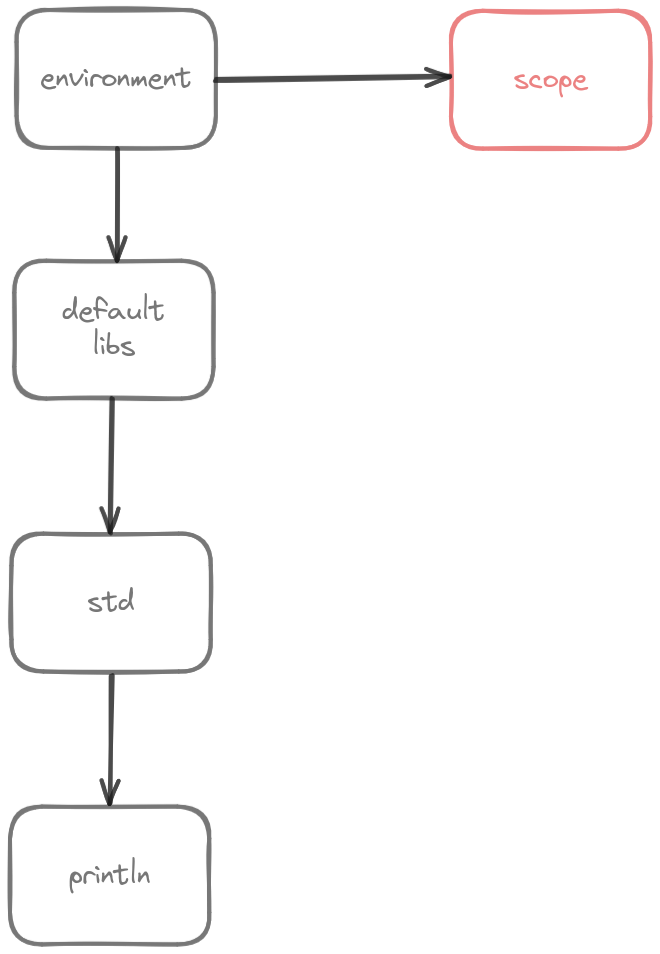
\includegraphics[scale=0.4]{ex-env-0.png}
    \caption{Cấu trúc của môi trường ở giai đoạn 1}
\end{figure}

    Bắt đầu với câu lệnh đầu tiên, \texttt{set a: int = 5;}, bộ thông dịch đọc câu lệnh này, kiểm tra ngữ nghĩa thông qua bộ xử lý ngữ nghĩa, rồi bổ sung thông tin biến \texttt{a} vào môi trường. Môi trường lúc này sẽ có cấu trúc như sau:

\begin{figure}[H]
    \centering
    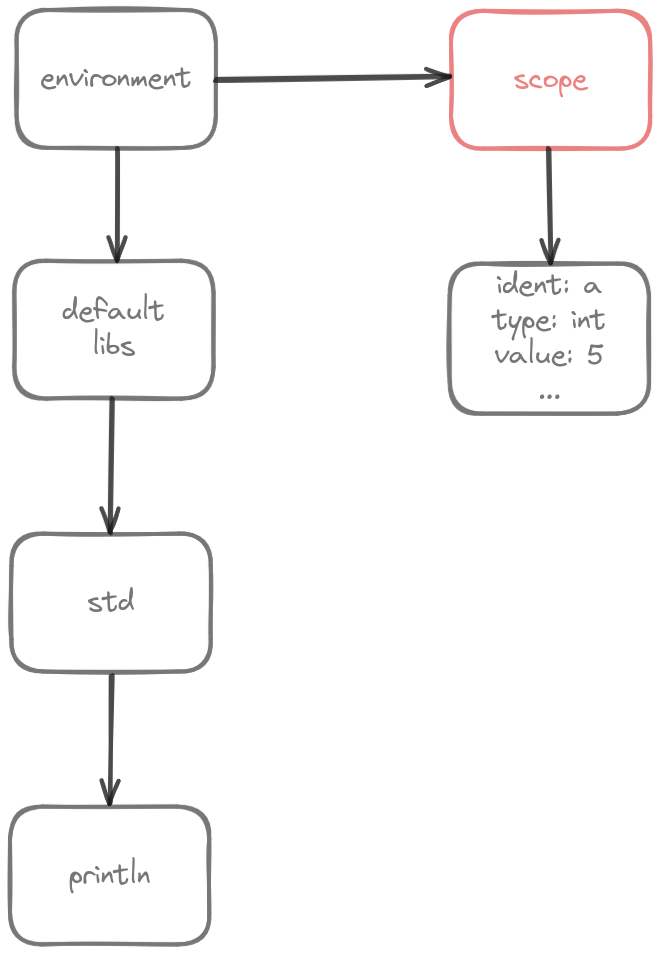
\includegraphics[scale=0.4]{ex-env-1.png}
    \caption{Cấu trúc của môi trường ở giai đoạn 2}
\end{figure}

    Tiếp theo, bộ thông dịch đọc câu lệnh gán \texttt{set b: int = a + 1;}. Khi đọc tới biến \texttt{a}, bộ xử lý ngữ nghĩa sẽ kiểm tra xem biến này có tồn tại trong môi trường hiện tại không. Khi phát hiện là biến có tồn tại và thấy ngữ nghĩa câu lệnh này hoàn toàn hợp lệ, bộ thông dịch tiến hành tính toán và cập nhật biến \texttt{b} vào môi trường hiện tại. Cấu trúc môi trường lúc này sẽ như sau:

\begin{figure}[H]
    \centering
    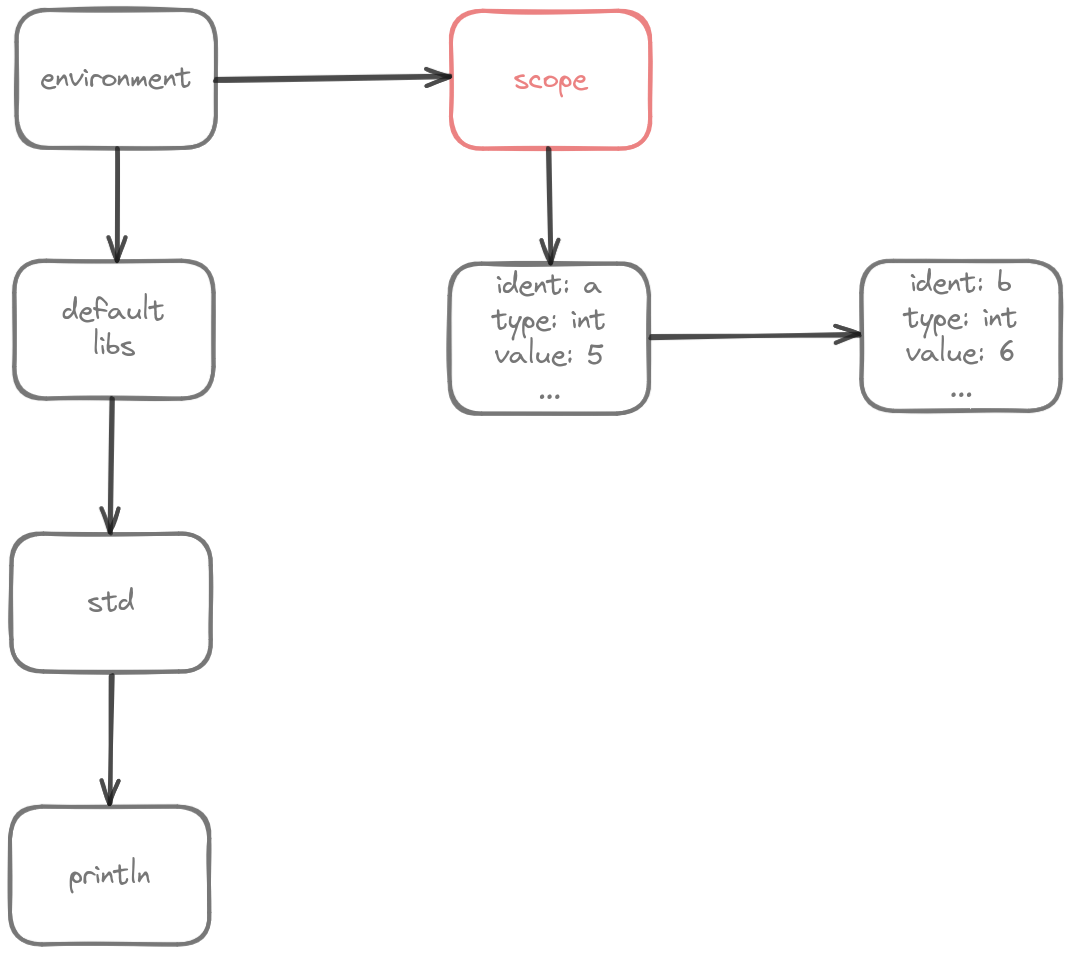
\includegraphics[scale=0.4]{ex-env-2.png}
    \caption{Cấu trúc của môi trường ở giai đoạn 3}
\end{figure}

    Bộ thông dịch đọc câu lệnh gán \texttt{set a: float = 3.14;}. Mặc dù biến \texttt{a} đã tồn tại trong môi trường, nhưng do ngôn ngữ Pandora cho phép shadowing, nên bộ thông dịch sẽ cập nhật thông tin biến \texttt{a} trong môi trường hiện tại. Lúc này, phạm vi hiện tại của môi trường sẽ chứa thông tin về hai biến \texttt{a} và thông tin biến \texttt{b} như sau:

\begin{figure}[H]
    \centering
    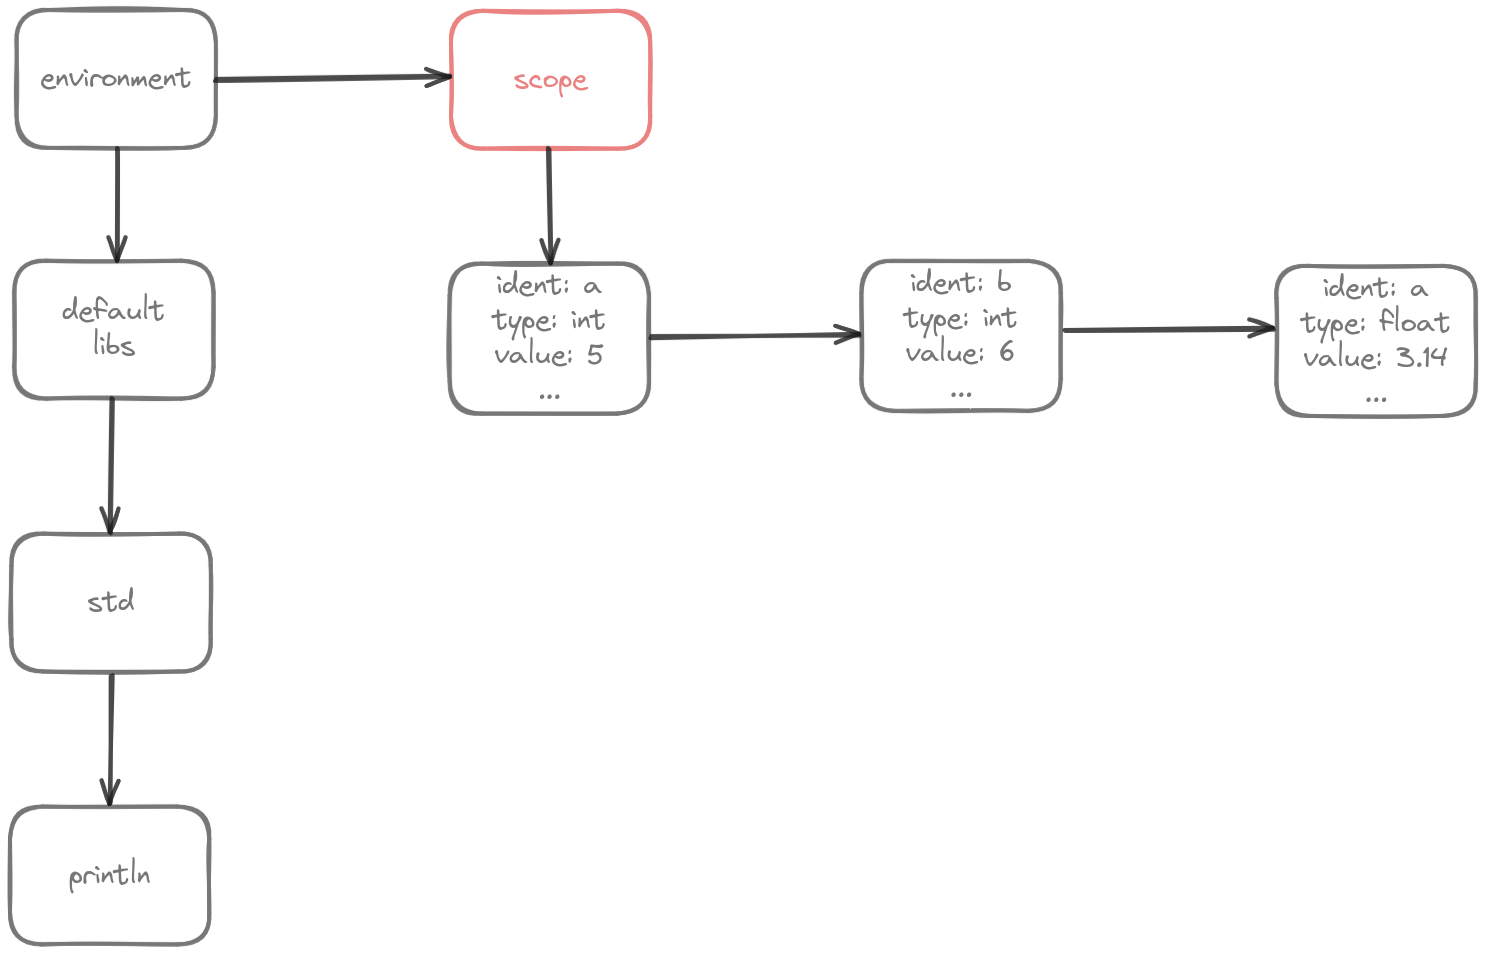
\includegraphics[scale=0.3]{ex-env-3.png}
    \caption{Cấu trúc của môi trường ở giai đoạn 4}
\end{figure}

    Sau đó, bộ thông dịch phát hiện câu lệnh tiếp theo là một khối lệnh, nên nó sẽ tạo một phạm vi mới và thêm vào danh sách phạm vi. Môi trường lúc này sẽ chứa thông tin về phạm vi hiện tại và phạm vi mới được tạo ra như sau:

\begin{figure}[H]
    \centering
    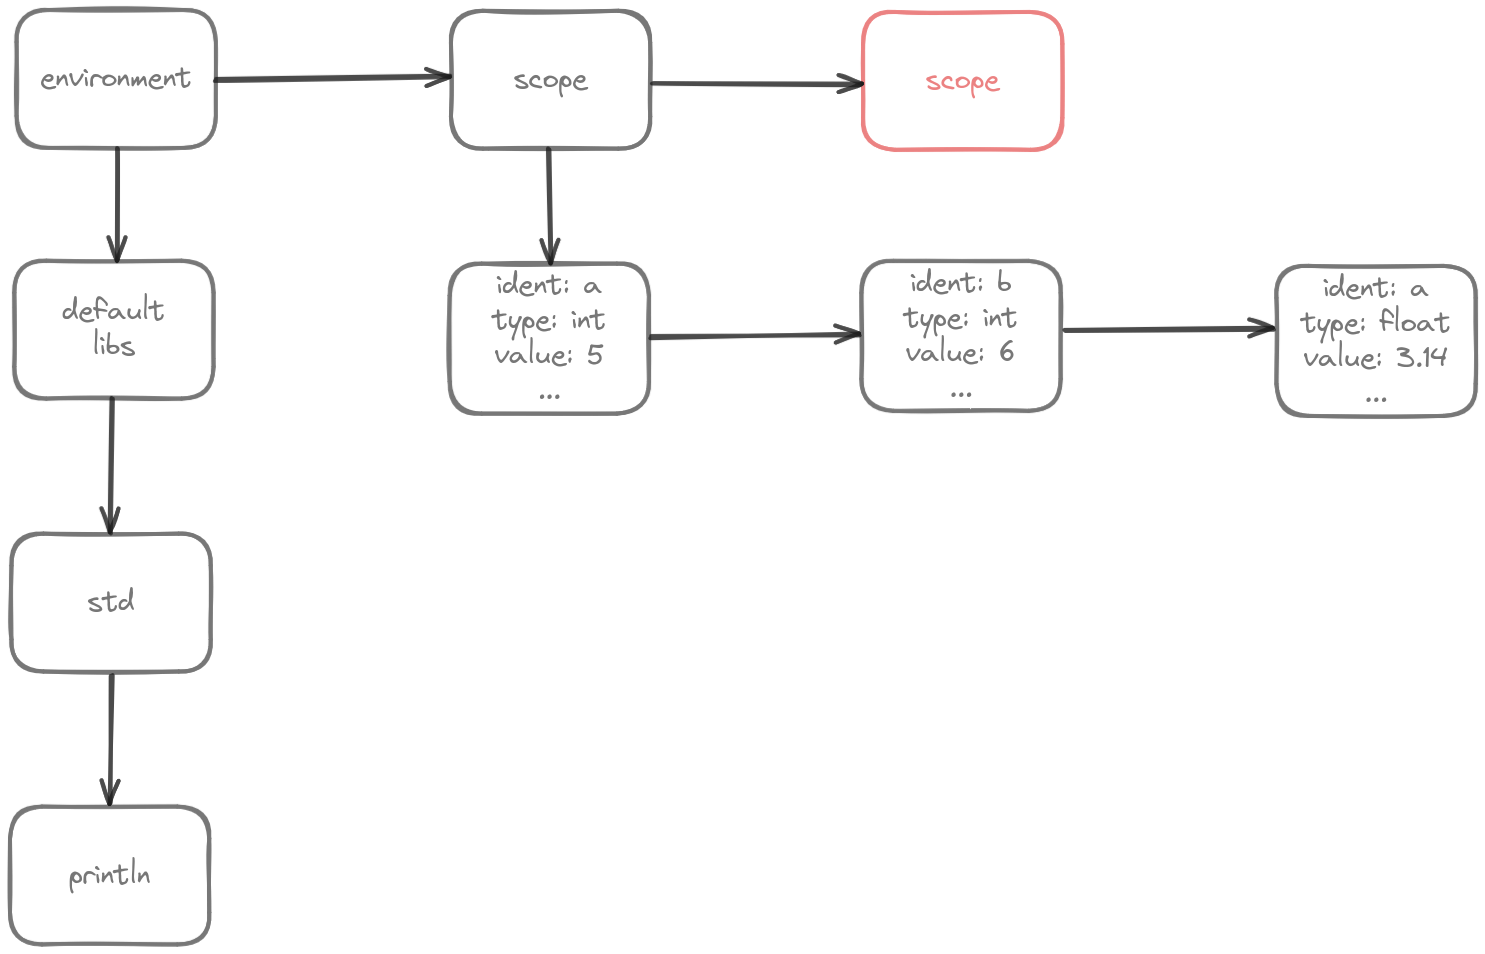
\includegraphics[scale=0.3]{ex-env-4.png}
    \caption{Cấu trúc của môi trường ở giai đoạn 5}
\end{figure}

    Câu lệnh đầu tiên trong khối lệnh là \texttt{set c: float = a - 1.1;}. Khi đọc tới biến \texttt{a}, bộ xử lý ngữ nghĩa sẽ kiểm tra xem biến này có tồn tại trong môi trường hiện tại hay không và tìm tháy thông tin về biến ở phạm vi trước đó. Lưu ý, môi trường sẽ lấy thông tin của biến ở phạm vi gần nhất mà nó tìm thấy. Nếu có nhiều biến trùng tên ở cùng một phạm vi, nó sẽ tiến hành lấy biến trùng tên đầu tiên tính từ phải sang trái(tức biến được thêm vào phạm vi sau cùng). Do vậy, với trường hợp trên, môi trường sẽ cung cấp thông tin về biến \texttt{a} có kiểu dữ liệuu là \texttt{float}. Sau khi kiểm tra ngữ nghĩa câu lệnh này, bộ thông dịch sẽ cập nhật thông tin biến \texttt{c} vào phạm vi hiện tại. Cấu trúc môi trường lúc này sẽ như sau:

\begin{figure}[H]
    \centering
    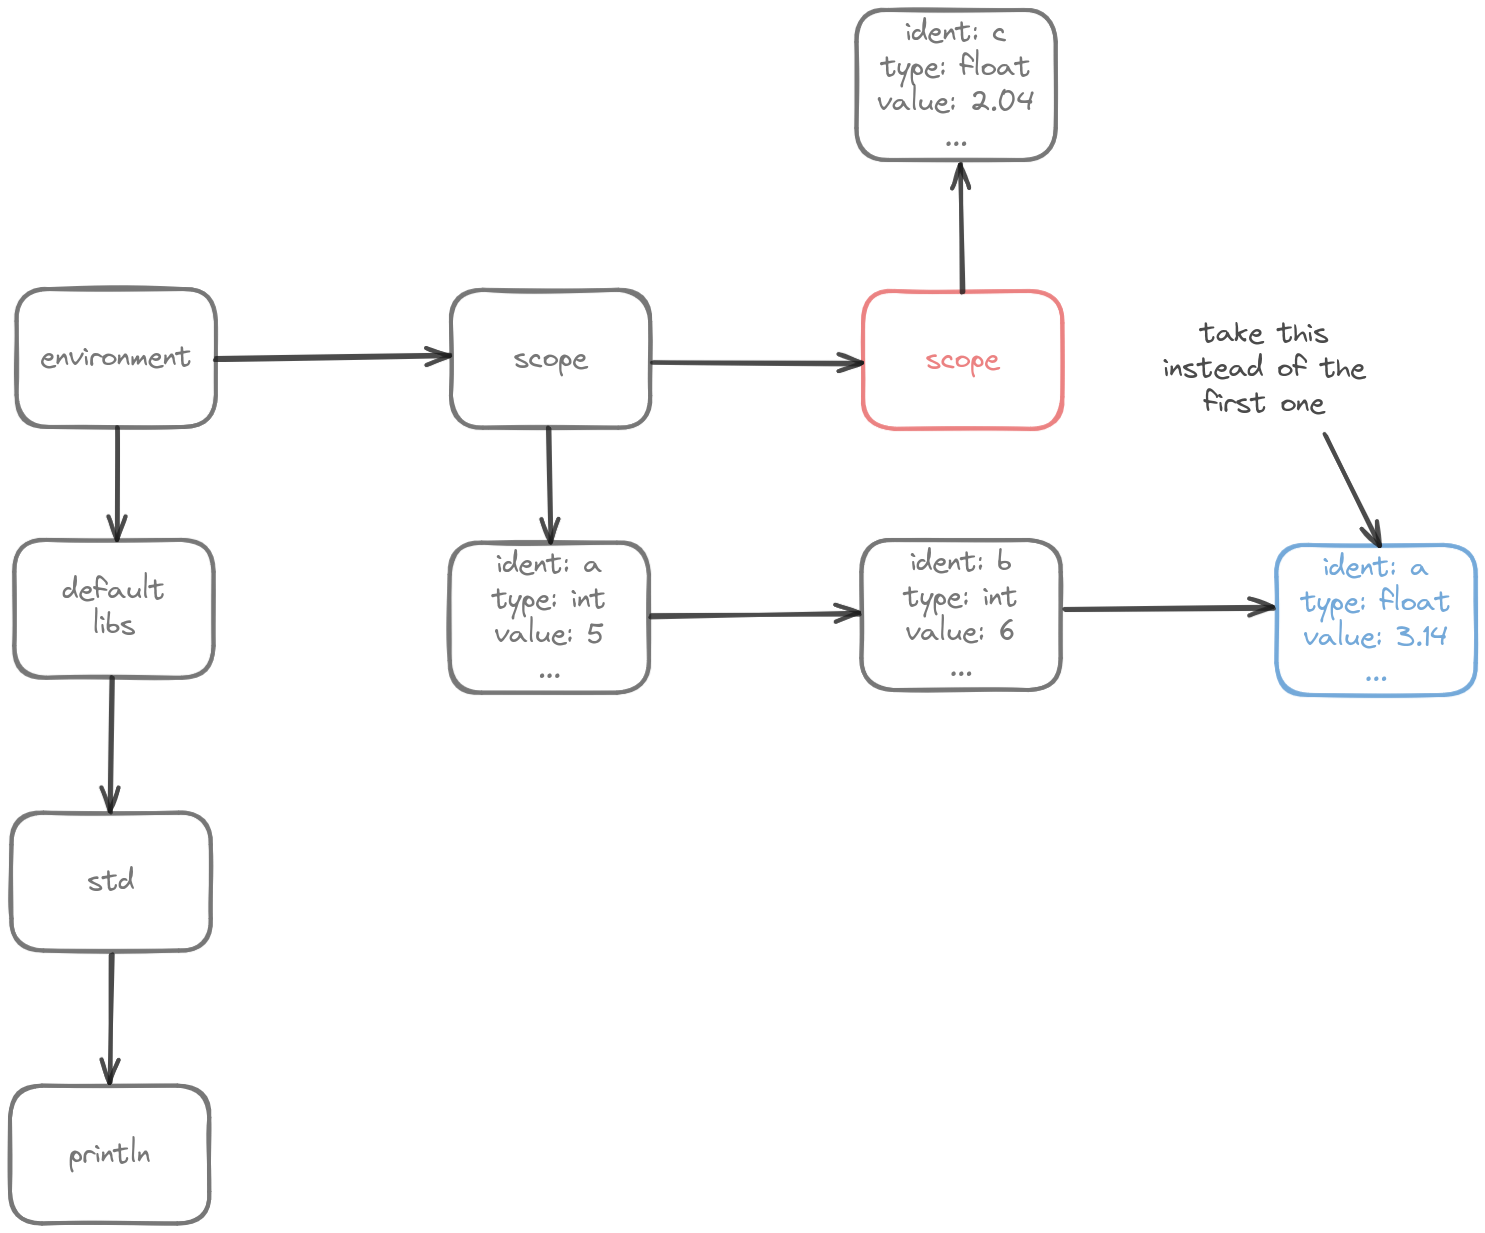
\includegraphics[scale=0.3]{ex-env-5.png}
    \caption{Cấu trúc của môi trường ở giai đoạn 6}
\end{figure}

    Tiếp theo, bộ thông dịch bắt gặp câu lệnh \texttt{println(c as str);}. Ở câu lệnh này, bộ thông dịch cần phải kiểm tra xem biến \texttt{c} và hàm \texttt{println} đã được khai báo hay thêm vào phạm vi hiện tại chưa. Biến \texttt{c} đã được khai báo trong phạm vi hiện tại, còn hàm \texttt{println} tuy chưa tồn tại trong phạm vi nào, nhưng lại nằm trong thư viện mặc định của Pandora, nên bộ thông dịch sẽ tiến hành thực hiện câu lệnh này. Kết quả sẽ được in ra màn hình là \texttt{2.04}.

    Sau khi thực hiện xong khối lệnh, môi trường sẽ xóa phạm vi cuối cùng khỏi danh sách phạm vi. Cấu trúc môi trường lúc này sẽ như sau:

\begin{figure}[H]
    \centering
    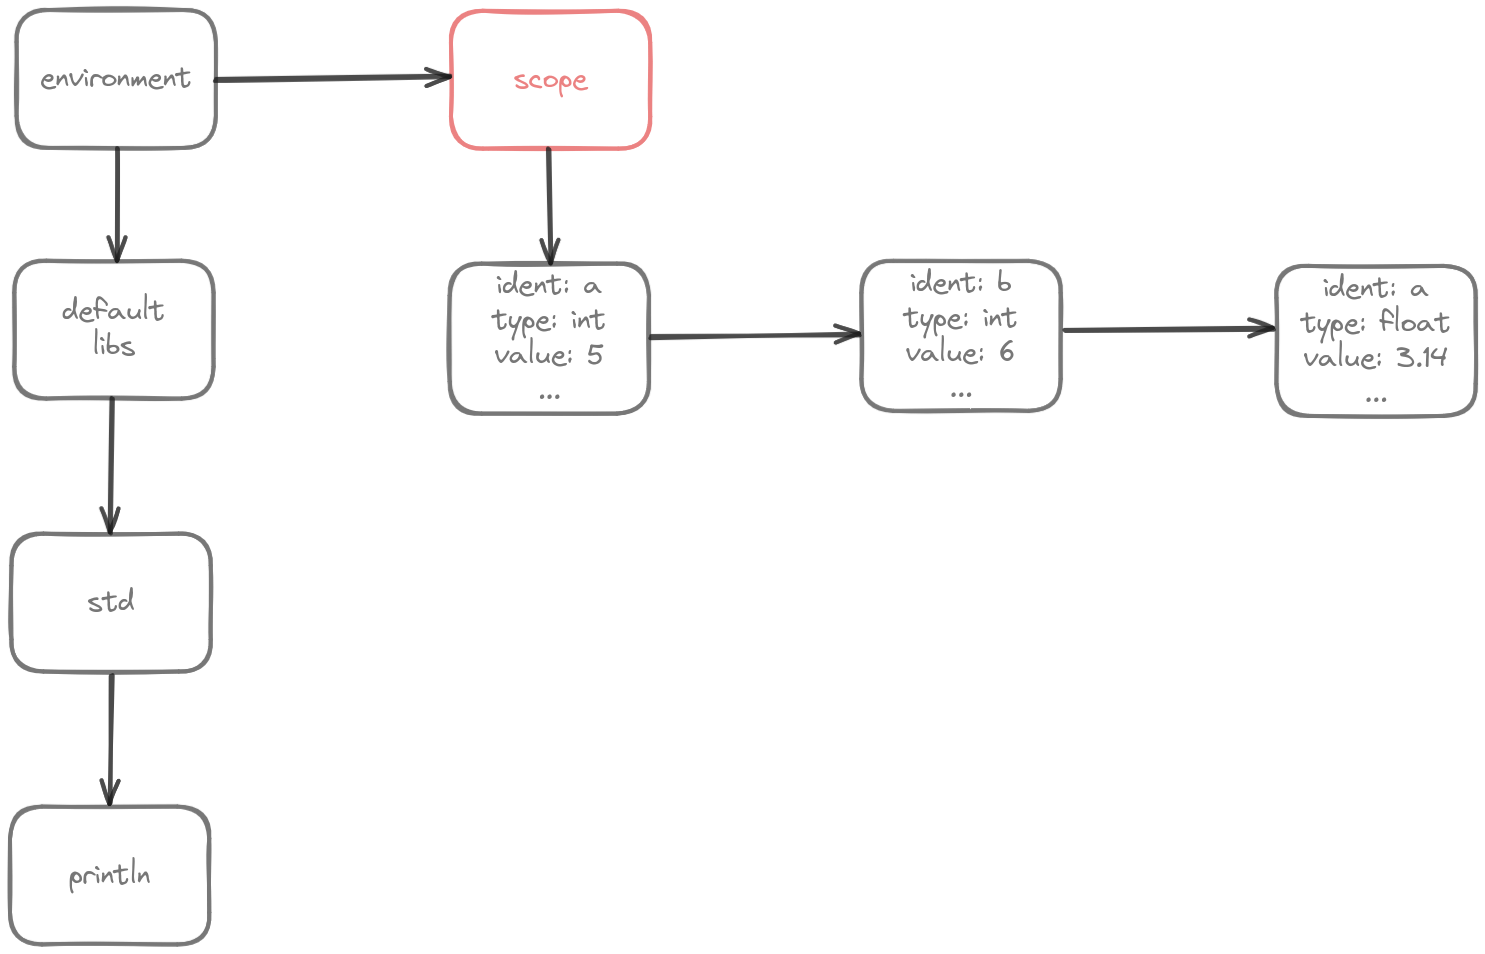
\includegraphics[scale=0.3]{ex-env-6.png}
    \caption{Cấu trúc của môi trường ở giai đoạn 7}
\end{figure}

    Với câu lệnh cuối cùng, \texttt{println(c as str);}, bộ thông dịch sẽ kiểm tra xem biến \texttt{c} và hàm \texttt{println} đã được khai báo hay thêm vào phạm vi hiện tại chưa. Tuy nhiên, môi trường không thể tìm thấy biến \texttt{c} trong phạm vi hiện tại, do biến này đã bị xóa khi ra khỏi khối lệnh trước đó. Do đó, bộ thông dịch sẽ báo lỗi và dừng chương trình.

    Với cách xây dựng môi trường như trên, trình thông dịch Pandora sẽ dễ dàng kiểm tra xem một biến, thư viện hay hàm đã được khai báo hay thêm vào phạm vi chưa, cũng như lấy thông tin về chúng một cách nhanh chóng. Đồng thời, việc sử dụng môi trường cũng giúp trình thông dịch Pandora duy trì thông tin về các biến, thư viện và hàm trong quá trình thực thi chương trình.
